\mainsection{4}{Dense Neural Networks }{05/05/2020}

A general model for $ q (\underline{y} | \underline{x} ; \Theta ) \\
$
*) can learn any linear or nonlinear mapping  \\
*) suitable for both regression and classification problems \\
artificial NN: mimic biological NN (brain)
\section{Fully connected neural networks - Neuron}
\putfigure{1.0}{1}{0.4}{Images/vlc_9n6oQpeN9Q}{Neuron}
\section{Chapter 4.2 Layer of Nurons}
\putfigure{1.0}{1}{0.4}{Images/vlc_AU8hElxhfe}{Layer of Neurons}\\
2 meanings of $\phi ()$: \\
\putfigure{1.0}{1}{0.4}{Images/vlc_sWrXTyRkHo}{Meanings of phi} \\
Comments : \\
\textbullet no interconnections between neurons in the same layer \\
\textbullet dense layer, fully connected layer:
\qquad \textbullet each input $ x_j$ connected to each neuron $i$ \\
$\rightarrow$ $c \cdot d$ weights and $w_ {ij }$ an c biases $b_i$ , $1 \leq i \leq c, 1 \leq j \leq d$, \\
$\rightarrow$ $ c \cdot (d+1)$ parameters
\section{Feedforward neural network}
A cascade of dense layers \\
\textbf{Layer } $ 1 \leq l \leq L:$ \\
$M_l -1 $ number of the input neurons \\
\putfigure{1.0}{1}{0.4}{Images/vlc_0aZPmMALw3}{Feedforward multilayer neural network} \\
\putfigure{1.0}{1}{0.4}{Images/vlc_doexEBUTyy}{Network Parameters}  \\


\section{Activation function}
Mild requirements on $ \phi() $: \\
\textbullet nonlinear in general $ \rightarrow $ fundamental \\
\textbullet smooth, differentiable $ \rightarrow $ for training \\
\textbullet simple calculation $ \rightarrow $ low complexity \\
\textbullet Slides 4-6; 4-7 activation function types \\

\subsection{Sigmoid activation function}
$ \phi (a) = \sigma (a) = \dfrac{1}{1 + e^{-a}} $ 
\putfigure{0.5}{1}{0.3}{Images/SigmoidActivationSketch.png}{Sigmoid function} \\
%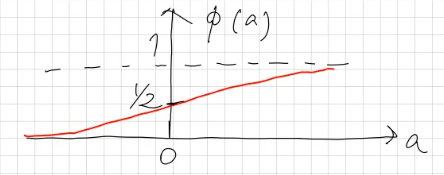
\includegraphics[width=0.5 \linewidth]{Images/SigmoidActivationSketch.png}\\
\textbullet $  0 < \phi < 1 \overset {\hat{}}{=}  $ prob.\\
\textbullet symmetry: $ \phi(-a) = 1-\phi(a)  $ \\
\textbullet derivative: $ \dfrac{d \phi(a) }{da} = ... = \dfrac{e^{-a}}{(1+ e^{-a})^2}  = \phi (a) \cdot \phi (-a ) = \phi (a) (1- \phi (a) ), \in (0,1) $\\
easy calculative \\
\textbullet widely used in conventional NN (shallow) \\
\subsection{hyperbolic tangent activation function }
$ \phi (a) = tanh(a) = \dfrac{e^{a} -e^{-a}  }{e^{a}  + e^{-a} }    $ \\
\putfigure{1.0}{1}{0.4}{Images/HyperbolicTangentActivation.png}{HyperbolicTangentActivation} 
%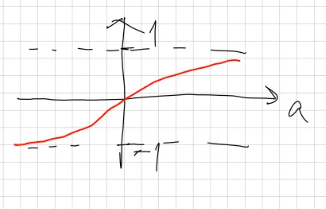
\includegraphics[width=\linewidth]{Images/HyperbolicTangentActivation.png} \\
like sigmoid but another output range 
\subsection{rectifier linear unit(ReLU}
$  \phi (a ) = ReLU(a) = max (a,0) =  \left\lbrace \begin{array}{lc}
a & a \geq 0 \\
0 & a < 0 
\end{array} \right.$ 
\putfigure{0.5}{0.7}{0.3}{Images/ReLuActivation}{ReLuA ctivation Function} 
%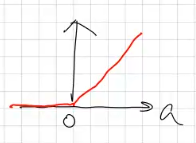
\includegraphics[width=\linewidth]{Images/ReLuActivation.png}\\
\textbullet $ \equiv $ diode \\
simple calculation \\
\textbullet $  \dfrac{d \phi}{da} = \left\lbrace \begin{array}{lc}
1 & a > 0 \\
0 & a <0 
\end{array} \right.  = u(a), u(0) = 0$ typically used \\
\textbullet most popular in DNN \\
\textbullet Details on 4-7
\subsection{Softmax activatoin function(classification problem)}
$  \phi (\underline{a} : \underline{a}  = [a_i ] \in \Re^c \rightarrow \Re^c$ \\
$  \phi ( \underline{a}) = softmax (\underline{a}) = \left[
\begin{matrix} 
\  \phi_1 (\underline{a}) \\
\vdots \\
\phi_c (\underline{a})
\end{matrix} \right] $ \\
$ \phi (\underline{a}) = \dfrac{ a^{a_i}}{\sum_{j=1}^{c} e^{a_i }} , \in (0,1) , \sum_{i=1}^{c} \phi_i (\underline{a}) = 1 $ \\
\textbullet maps $  \underline{a} \in \Re^c  $ to a categorical PMF with $ c $ classes  \\
\textbullet $  a_i  $ large$  \rightarrow \phi_i (\underline{a} )  $ close to 1 \\
\textbullet $  a_i  $ small $ \rightarrow \phi_i (\underline{a} )  $ close to 0 \\
\textbullet used in the output layer for classification problems \\
\subsection{Special case c=2, binary classification problem}:
$ \phi_1 (\underline{a}) = \dfrac{e^{a_i}}{e^{a_1} + e^{a_2}} = \dfrac{1}{1+ e^{-(a_1 - a_2)}} = \sigma (a_1 - a _ 2) \\
\phi_2 (\underline{a} = \dfrac{e^{a_2}}{e^{a_1} + e^{a_2}} = 1 - \phi_1 (\underline{a}) = \sigma (a_2 - a_1) \\
$
i.e. softmax \\
\putfigure{1.0}{1}{0.1}{Images/OutputLayerSoftmax.png}{Outputlayer Softmax} 
%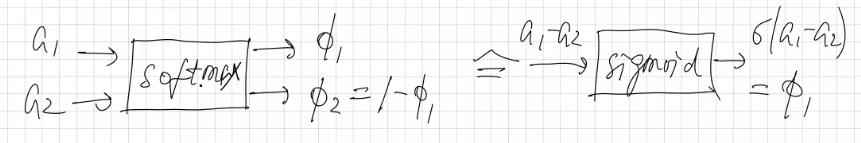
\includegraphics[width=\linewidth]{Images/OutputLayerSoftmax.png} \\
one sigmoid output is sufficient for binary classification instead of 2 output softmax! \\
\textbf{  Derivative of softmax:}\\
$ \dfrac{ \partial \phi_i (\underline{a}) }{\partial a_j} = ... = \left\lbrace \begin{array}{lc}
\phi:i (\underline{a})\cdot ( 1- \phi_i (\underline{a}) & i=j \\
- phi_i (\underline{a}) \cdot \phi_j (\underline{a}) & i \neq j 
\end{array} \right. $
\textbullet 4-9 for details on usage \\
\section{Universal approximation } 
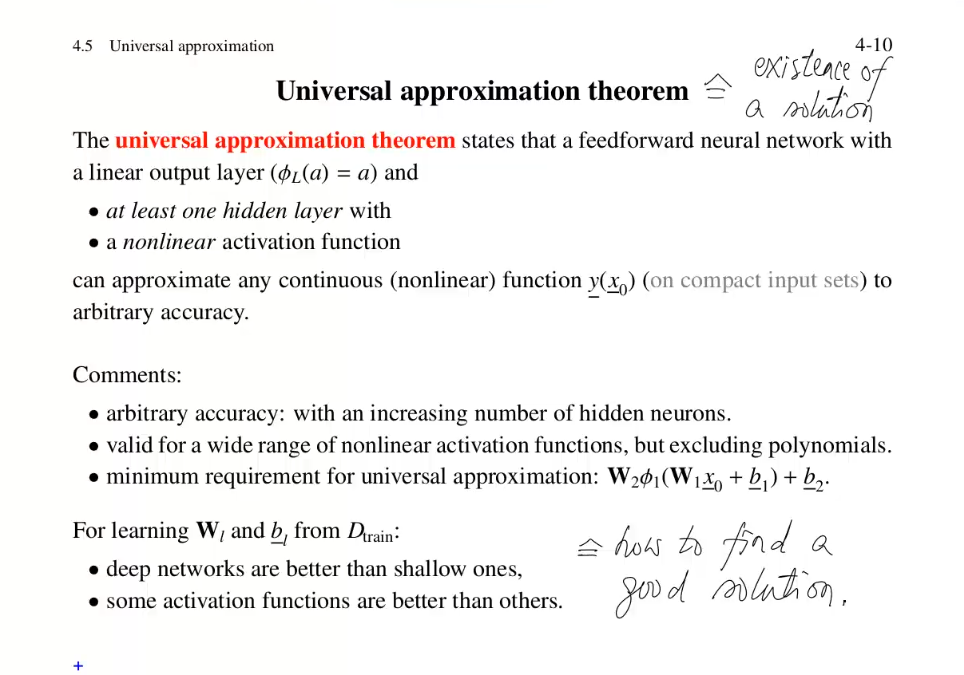
\includegraphics[width=\linewidth]{Images/Slide410.png}

\subsection{E4.3 Regression with 1 hidden layer}
True function: $ f_0(x)   $\\
Given: $ x(n)  $ and noisy function $ y(n) = f_(x(n)) + z(n) , 1 \leq n \leq N  ,z(n)$ is the noise \\
NN: \\
\putfigure{1.0}{1}{0.4}{Images/E43Architecture.png}{Example 4.3 Architecture} 
%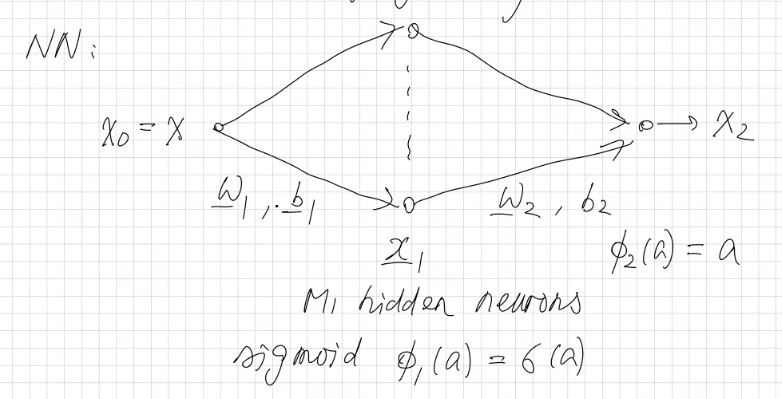
\includegraphics[width=\linewidth]{Images/E43Architecture.png}\\
i.e. $  x_2 = f(x, \underline{\theta}) = \underline{w}_2^T \sigma ( \underline{w}_1 x + \underline{b}_1 )  $, column times row times scalar \\
$ = \sum_{i=1}^{N_1} w_{2,i} \cdot \underbrace{\sigma ( w_{1,i} x + b_{1,i}) }_{M_1 \text{ nonllinear basis functions of }x} + b_2$ \\
$ \sigma ( w_i x + b_i ) \sigma (w_i ( x + \dfrac{b_i}{w_i})) $ \\
new center at $ \dfrac{-b_i}{w_i} $ and new slope value $ w_i $ \\
Picture is for black 1 $ w_i $ red another $ w_i $ green another example $ w_i $\\
\putfigure{1.0}{1}{0.2}{Images/E43Sketchsigmoid}{Sketch for sigmoid} 
%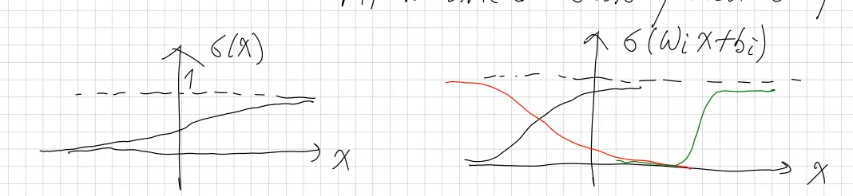
\includegraphics[width=\linewidth]{Images/E43Sketchsigmoid.png}
\section{Loss and cost function}
\textbf{Review chapter 3.4}	\\
\putfigure{1.0}{1}{0.15}{Images/ProbabalisticFrameworkSupervisedLearning}{Probabalisitc Framework supervised learning} 
%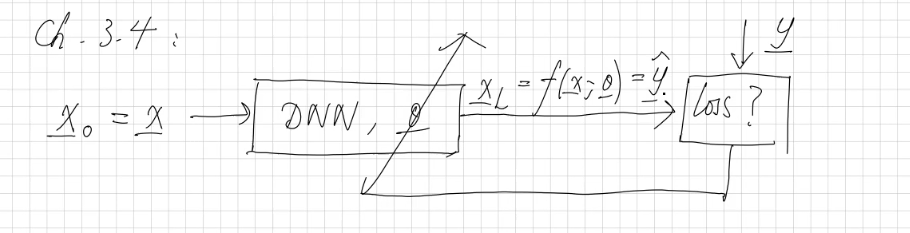
\includegraphics[width=\linewidth]{Images/ProbabalisticFrameworkSupervisedLearning.png}\\
$ \underset{\underline{\theta}}{min}  L ( \underline{\theta  }) =  \dfrac{1}{N} = \sum_{n=1}^{N} (l(\underline{x}(n), y(n)_i \underline{\theta}$     cost function for $ d_{train } $ \\
$l(\underline{x}, \underline{y}_j \underline{\theta }) = - ln(q ( \underline{y} | \underline{x}_j \underline{\theta } )  $ loss for one pair $  (\underline{x}, \underline{y})  $ \\
$  q () \leftrightarrow $ DNN ???
\subsection{Regression Problem}
$ \underline{x} \in \Re^d $: random input \\
$ \underline{y} \in \Re^c $ desired random output \\
Assumption: DNN estimates the mean of $ \underline{y} $, i.e. \\
$  \underline{y} = f(\underline{x} , \underline{\theta})  + \underline{z} , \underline{z}$ : noise \\
f is calculated by DNN \\
\textbf{case A: } : $  \underline{z} \sim N(\underline{0} , \sigma^2 \underline{\underline{I}}),$ white Gaussian noise\\
$ \underline{y} \sim N(f(\underline{x}, \underline{\theta}), \sigma^2 \underline{\underline{I}}  ) $\\
$ q (\underline{y} | \underline{x} , \underline{\theta}) = \dfrac{1}{(2 \pi \sigma^2)^{c/2}}  exp ( \dfrac{-1}{2 \sigma^2} || \underline{y} - f(\underline{x}, \underline{\theta) ||^2})$ \\
$ l(\underline{x}, \underline{y} , \underline{\theta})  = -ln (q(\underline{y}| \underline{x} , \underline{\theta})) = const.+ \dfrac{1}{\sigma^2} || \underline{y} - f(\underline{x} , \underline{\theta}) ||^2\\
L(\underline{\theta}) = \dfrac{1}{N} \sum_{n=1}^{N} || \underline{y}(n) - f(\underline{x} , \underline{\theta}) ||^2 \\
\rightarrow l_2- loss, $ mean square error (MSE) loss , least squares (LS) method \\
min $ L(\underline{\theta}) $ is a parameter estimation problem \\
\textbf{ case B:} \\
$ \underline{z} \sim N(\underline{0} , \underline{\underline{C}}) ,  $ colored Gaussian noise \\
$ L(\underline{\theta})  = \dfrac{1}{N} \sum_{n=1}^{N} [\underline{y} - (f(\underline{x}(n) , \underline{\theta})]^T \cdot \underline{\underline{C}}^{-1} \cdot [\underline{y} - (f(\underline{x}) , \underline{\theta})] $ , \textbf{weighted MSE loss}\\
Rarely used in real life applications: \\
\textbullet how to know $ \underline{\underline{c}} $ \\
\textbullet $ \underline{\underline{C}}^{-1} $ expensive for large $ \underline{\underline{C}} $ \\
\subsection{Classification}
$ \underline{x} \ in \Re^d  $: input \\
$ \underline{y} \in \lbrace \underline{e}_1 , \underline{e}_2,..,\underline{e}_c \rbrace $ \\: class label for $ \underline{x} $ in one-hot coding \\
Let $ p_i = P(\underline{y} = \underline{e}i | \underline{x} )  $: true posterior probability \\
ch: 3.2 : $ P(\underline{y} | \underline{x}) = \prod_{i=1}^{c}  p_i ^{y_i}$ true PMF \\
But $ p_i $ unknown \\
\textbf{DNN: }
\textbullet output $ f(\underline{y} ,\underline{\theta}) = [f_i (\underline{x}; \underline{\theta})] \in \Re^c $ an estimate for $  [p_i]  $ \\
\textbullet i. e. $ P(\underline{y} | \underline{x}) $ approximated $ Q (\underline{y} | \underline{x} ; \underline{\theta})  = \prod_{ i=1 }^{c} f_i ( \underline{x} ; \underline{\theta})^{y_i}$\\
in order to ensure : \\
\textbullet $  0 < f_i (\underline{y} ; \underline{\theta}) < 1 \\ $\\
\textbullet $  \sum_{i=1}^{c} f_i (\underline{x} ; \underline{\theta})  = 1,$ \\
softmax is used in the output layer : \\
$  \underline{x} _{L} = f (\underline{x} ; \underline{\theta}) = \phi_L (\underline{a}_lL) = softmax (\underline{a}_L) , $ see ch.4.4\\
$  \rightarrow \text{ Loss } l(\underline{x} , \underline{y} ; \underline{\theta}) = - ln(Q(\underline{y} | \underline{x} ; \underline{\theta })) = \sum_{i=1  }^{c} y_i ln (f_i (\underline{y} ; \underline{\theta}))   = - \underline{y} ^T ln (f(\underline{x} ; \underline{ \theta })) \geq 0 $\\
categorical cross entropy(CE) loss \\
Special case : Binary classification , c = 2 \\
ch.4.4: $ softmax , c = 2 \leftrightarrows sigmoid $ \\
i.e. one output neuron with sigmoid activation function $ f(\underline{x}; \underline{ \theta})  = \sigma (a_L)$ is sufficient\\
Let $  y_1 = y, y_2 = 1 - y ; f_1 = f ; f_2 = 1-f $ \\
$ \rightarrow l(\underline{x} , \underline{y} ; \underline{\theta}) = - y ln(f(\underline{x}; \underline{\theta}) + (1-y)) \cdot ln(1-f(\underline{x}; \underline{\theta})) $ , binary CE loss \\
\textbf{True probabilistic way toward cost functions}\\
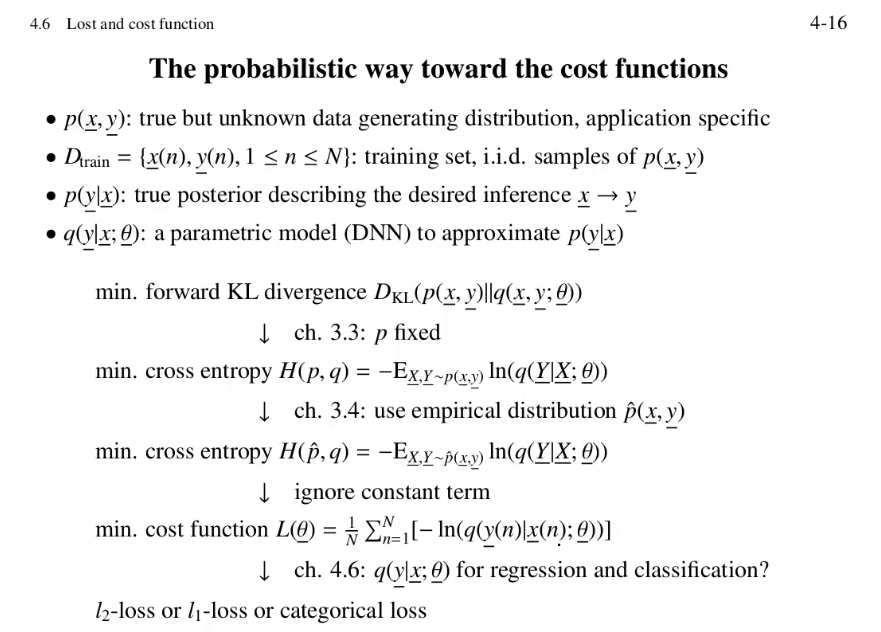
\includegraphics[width=\linewidth]{Images/ProbabalisticWayCostFunction.png}\\
\subsection{Semantic segmentation }
\textbf{pixelwise classification }\\
categorical cross entropy loss: \\
$  l(\underline{\underline{X}} , \underline{\underline{Y}}; \underline{\theta}) = \sum_{m=1}^{M} \sum_{n=1}^{N}[- \underline{y}_{mn} \cdot ln (\hat{\underline{y}}_{mn} ( \underline{\underline{X}}, \underline{\theta} )) ] $
sum over all pixels\\
Problem: imbalanced classes \\
e.g (c=2) background and foreground with 90 \% background and 10 \% foreground pixels , 90 \% loss function for the foreground \\
$\rightarrow l(\cdot)$ cares more about the major class and less about the minor class but the minor class(foreground) is object of interest. 
$\rightarrow$ reduced segmentation accuracy for the minor class \\
\textbf{Solutions:} \\
\textbullet Weighted categorical CE loss \\
\textbullet region-based loss 
\textbf{Jaccard index only used for result evaluation not suitable as loss function for training}\\
\textbullet minimize loss, not max J or D for those indexes\\
\textbullet $ |A|  \in \N$, not differential with respect to $ \underline{\theta} $\\
\textbullet $ \underline{y}_{mn} $ contains 0 or 1 as desired, but $ \hat{\underline{y}}  $ contains real numbers $ \in (0,1) \in softmax $ \\
$\rightarrow$ adapted definition of J and D are necessary \\
\putfigure{1.0}{1}{0.4}{Images/SoftJaccardDiceLoss}{Soft Jaccard / Dice loss} 
%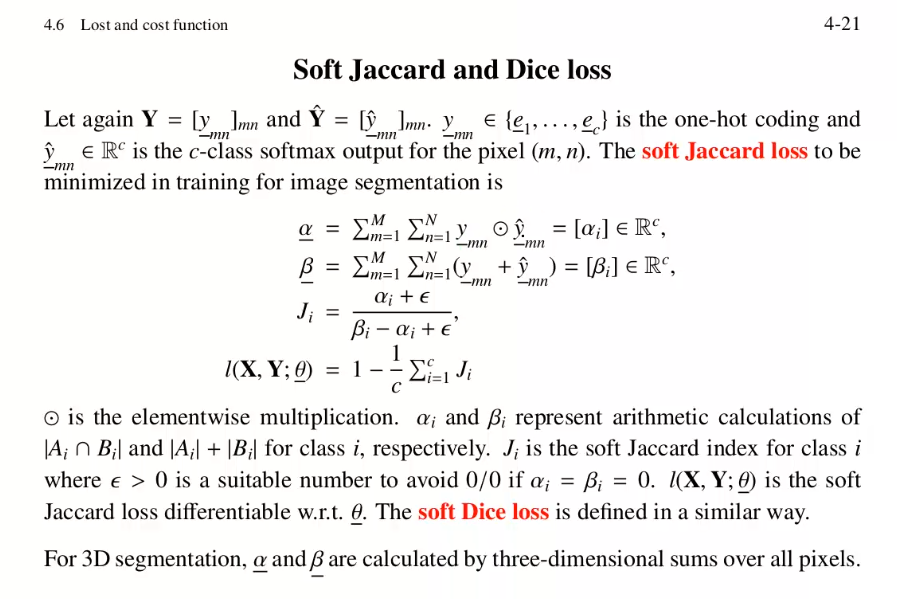
\includegraphics[width=\linewidth]{Images/SoftJaccardDiceLoss.png}\\
\textbf{Very good for strongly imbalanced classes }
\section{Training}
\textbullet training set $ D_{train} = \lbrace \underline{x} , \underline{y } , 1 \leq n \leq N \rbrace $\\
\textbullet cost function $ L(\underline{\theta}) = \dfrac{1}{N} \sum_{n=1}^{N} l(\underline{x}(n),\underline{y}; \underline{\theta}) $ \\
\textbullet task: $ min L(\underline{\theta}) $\\
\textbullet optimizer: optimization algorithm to solve the minimization task $ L(\underline{\theta}) $ \\
No closed-form solution! Numerical minimization necessary, see AM (last part) \\
\textbf{in DL: gradient decent approach and variants(like hiking)}\\
need only 1. order derivative of $ L(\underline{\theta}) $ \\
\putfigure{1.0}{1}{0.4}{Images/GradientDescent}{Gradient descent} 
%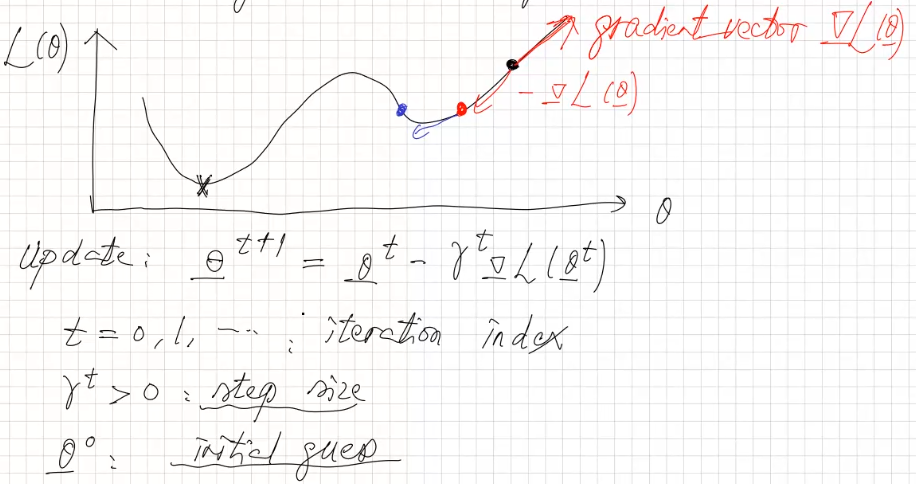
\includegraphics[width = \linewidth]{Images/GradientDescent.png}\\
calculation of the gradient vector $  \underline{\nabla} L(\underline{\theta}) $ is non trivial \\
\subsection{Chainrule of derivative (back propagation)} 
$\dfrac{ f(g(\theta))}{d \theta} = \dfrac{df}{dg} \cdot \dfrac{dg}{d \theta} $ \\
Layerindex L: $  \dfrac{\partial L_{cost}(\underline{\theta})}{\partial w_{L,ij}} = \dfrac{\partial L_{cost} }{\partial \underline{x}_{L}} \cdot \dfrac{\partial \underline{x}_K}{\partial \underline{a}_L} \cdot \dfrac{\partial \underline{a}_L }{\partial w_{L,ij}} = \underbrace{ \underline{\underline{J}}_L (\underline{x}_L) \cdot \underline{\underline{J}}_{\underline{x}_L}(\underline{a}_L)}_{\underline{\underline{J}}_L (\underline{a}_L)} \cdot \underline{\underline{J}}_{\underline{a}_L} (w_{L,ij}) $, Jacobi matrices see ch. 3.1\\
Notation: $ \underline{\underline{J}}_y (x ) = \dfrac{\partial y}{\partial x}  $ \\
Layer $ L-1$:\\
$ \dfrac{\partial L (\underline{\theta})}{\partial w _{L-1, ij}} = \dfrac{\partial L}{\partial \underline{a}_L} \cdot \dfrac{\partial \underline{a}_L}{\partial \underline{a}_{L-1}} \cdot \dfrac{\partial  \underline{a}_{L-1}}{\partial w_{L-1,ij}} = \underbrace{ \underline{\underline{J}}_L (\underline{a}_L) \cdot \underline{\underline{J}}_{\underline{a}_L} (\underline{a}_{L-1})}_{\underline{\underline{J}}_L(\underline{a}_{L-1})} \cdot \underline{\underline{J}}_{\underline{a}_{L-1}}(w_{L-1,ij}) $ \\
Layer 1: $ \dfrac{\partial L (\underline{\theta})}{\partial w_{1,ij}} = \underline{\underline{J}}_L ( \underline{a}_L) \cdot \underline{\underline{J}}_{\underline{a}_L}(\underline{a}_{L-1}) , ..., \underline{\underline{J}}_{\underline{a}_2}(\underline{a}_1) \cdot \underline{\underline{J}}_{\underline{a}_1} (w_{1,ij}) $ \\
\putfigure{1.0}{1}{0.4}{Images/Training423}{Forward pass vs. backward pass} 
%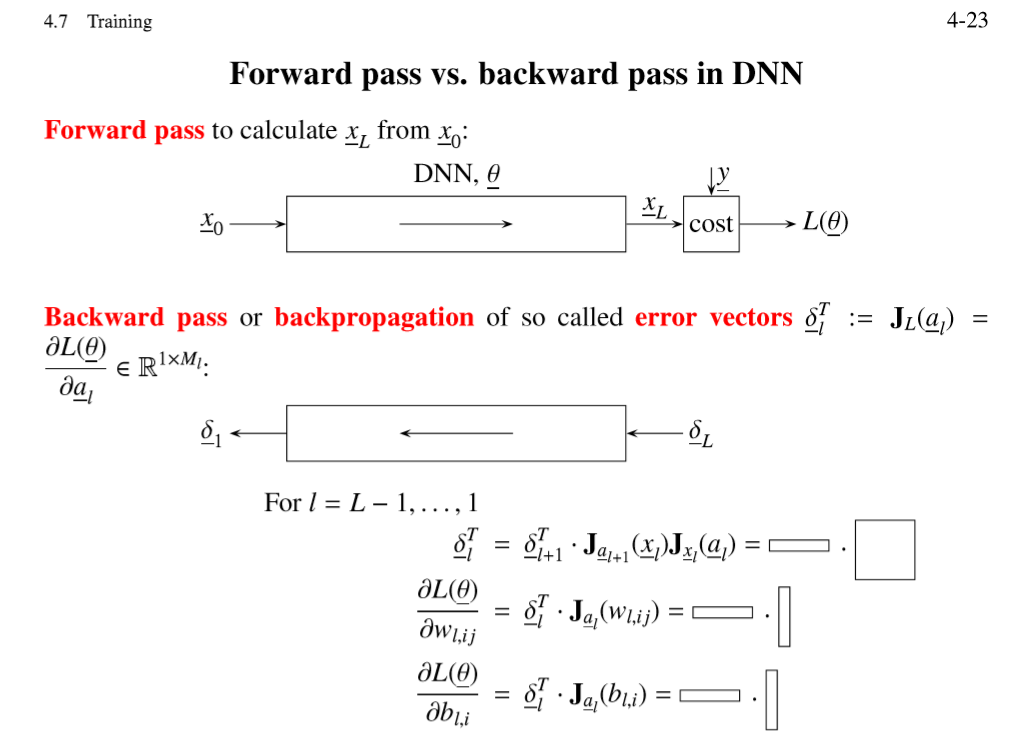
\includegraphics[width = \linewidth]{Images/Training423.png}\\
\textbf{Calculations for backpropagation on Slide 4-24 to 4-27}\\
more about omptimizer in ch.5 \\
more about model in ch. 6-8 \\
\textbf{Batch gradient descent }\\
calculate $  \underline{\nabla} L (\underline{\theta}) = \dfrac{1}{N} \sum_{n=1}^{N} \underline{\nabla } l(\underline{x}(n) , \underline{y} (n); \underline{\theta}) $ \\
for the whole training set $ D_{train} $ \\
Difficult for too large N!\\
e.g. MNIST: 60.000 training smaples \\
ILSVRC: 1.2M training samples \\
$\rightarrow$ not enough ram to keep $ D_{train} $ in memory \\
Solution: stochastic gradient descent (SGD), i.e. calculate $ \underline{\nabla}L $ and update $ \underline{\theta} $ for each minibatch, a block of B samples from $ d_{train} $: \\
$ \underline{\theta}^{t+1} = \underline{\theta}^t - \underline{\nabla}L (\mathbf(t); \underline{\theta})|_{\underline{\theta} = \underline{\theta}_t} $\\
$ L(t; \underline{\theta}) =  \dfrac{1}{B} \sum_{n=t'B+1}^{(t' +1) \cdot B} l (\underline{x}(n), \underline{y} ; \underline{\theta})$ \\
$  B \in \N: $ minibatch size, small enough to fit in RAM \\
$ N/B \ in \N:  $ number of minibatches in $ d_{train} $ \\
$  t = 0,1 ,..,  $: iteration index \\
$  t' = mod(t, \dfrac{N}{B}) \in \lbrace 0,1,.., \dfrac{N}{B-1} $: minibatch index \\
$  \underline{\nabla } L (t; \underline{\theta}) $ more noisy than $\underline{\nabla} L (\underline{\theta} )$\\
$\rightarrow$ stochastic gradient descents \\
\textbf{Evaluation during training:} \\
$  \hat{ \underline{\theta}}_k  $ after k-th epoch: $  k = 1,2,.. $ \\
\textbf{Technical performance metrics:}
\textbullet training loss: $  L(\hat{\underline{\theta}}_k) $ calculated form training set $ D_{train} $\\
\textbullet test loss::$ L(\hat{\underline{\theta}}_k) $ calculated form test set $ D_{test} $\\
and objective performance metrics for classification \\
\textbullet \textbf{training error rate :} Error rate of $ DNN( \hat{\underline{\theta}}_k) $ for $ D_{train} $\\
\textbullet \textbf{test error rate :} Error rate of $ DNN( \hat{\underline{\theta}}_k) $ for $ D_{test} $\\
or:
\textbullet training/test accuracy =   1- training/test error rate 
\section{4.8 Implementation of DNN's in Python}
\textbullet $ 60000/ 128 ) 468,795 \approx 469 $ mini-batches (slide 4-33)\\
\textbullet see python script KerasDemo